\documentclass[12pt,a4paper]{ctexart}
\usepackage{graphicx}
\usepackage{wrapfig}
\usepackage{float}
\usepackage{siunitx}
\usepackage{subfigure}
\usepackage{caption}
\usepackage{natbib}
\usepackage{listings} % 引入listings宏包用于插入代码
\usepackage{xcolor} % 引入xcolor宏包以支持更多的颜色设置

% 设置Verilog代码样式
\lstdefinestyle{verilog}{
    language=Verilog, % 设置语言为Verilog
    basicstyle=\small\ttfamily, % 设置基本字体样式
    keywordstyle=\color{blue}, % 关键字颜色设置
    commentstyle=\color{gray}\ttfamily, % 注释颜色和样式设置
    stringstyle=\color{red!60!black},
    numbers=left, % 行号在左边显示
    numberstyle=\tiny,
    frame=single, % 添加单线框
    rulecolor=\color{black!30}, % 边框颜色
    breaklines=true, % 允许自动换行
}
\begin{document}
\section*{$1$}
\subsection*{$1$}
\begin{figure}[h]
    \begin{center}
        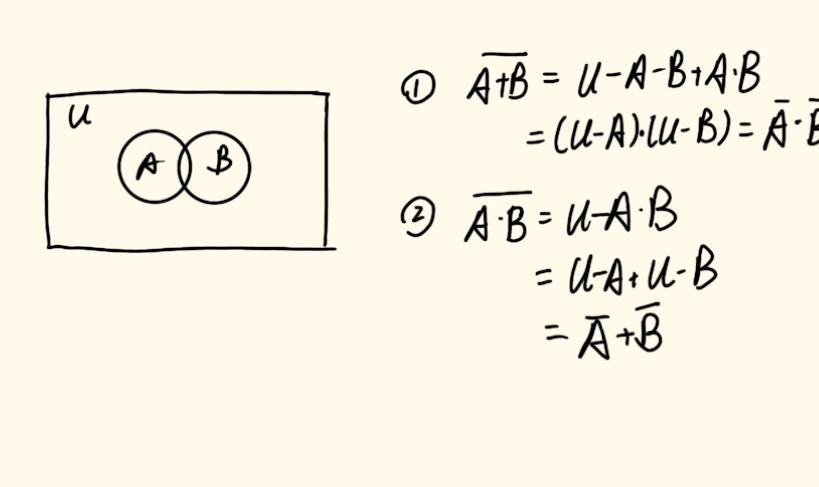
\includegraphics[scale=0.5]{Screenshot_20240321_171754_com.huawei.hinote.png}
    \end{center}
\end{figure}
\subsection*{$2$}
\begin{figure}[h]
    \begin{center}
        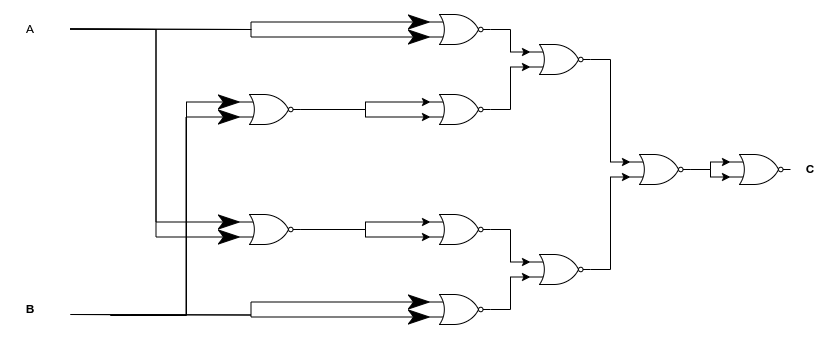
\includegraphics[scale=0.5]{未命名绘图.drawio.png}
    \end{center}
\end{figure}
\newpage
\section*{2}
\subsection*{1}
ALU是计算机CPU中的核心部件,负责执行基本的算术和逻辑运算。它能够对数据进行加、减、乘、除等算术操作,并执行与、或、非、异或等逻辑操作。\par
REG FILE是一个存储区域,包含一组可快速访问的寄存器。每个寄存器可以存储一定数量的位(例如32位或64位),用于暂存数据、计算中间结果或保存程序状态信息。通过读写寄存器,CPU可以在不同阶段高效地处理和传递数据。\par
MUX是一种数字电路元件,它的作用是在多个数据源之间进行选择,并将选定的数据通道传输到单一输出端。\par
MEMORY是计算机系统中的主要存储设备,用于长期存储程序和数据。它按照地址寻址的方式组织数据,允许CPU按需读取和写入数据。\par
\subsection*{2}
CPU内包含了ALU、REG FILE和MUX。
内存对应MEMORY。
\subsection*{3}
输入设备:键盘,鼠标;\par
输出设备:显示器,音箱。
\section*{3}
\subsection*{1}
$CPI=0.5\times1+0.4\times2.5+0.1\times5=2$
\subsection*{2}
$t=\frac{CPI}{f}=\frac{2}{f}s$
\subsection*{3}
$t=\frac{1.8}{f}s$
\subsection*{4}
即该程序$CPI$变为$1.8$,则乘法$CPI$变为$2$
\subsection*{5}
即该程序$CPI$变为$1.8$,则访存指令$CPI$变为$3$
\section*{4}
\subsection*{1}
<1> posedge clk
<2> q<=0x08;
<3> q<=d;
\subsection*{2}
执行复位操作
\subsection*{3}
<1> posedge clk or rst
\section*{5}
\subsection*{1}
\begin{tabular}{|c|c|c|c|c|}
    \hline
    A & B & Cin & Sum & Cout \\
    \hline
    0 & 0 & 0   & 0   & 0    \\
    \hline
    0 & 0 & 1   & 1   & 0    \\
    \hline
    0 & 1 & 0   & 1   & 0    \\
    \hline
    0 & 1 & 1   & 0   & 1    \\
    \hline
    1 & 0 & 0   & 1   & 0    \\
    \hline
    1 & 0 & 1   & 0   & 1    \\
    \hline
    1 & 1 & 0   & 0   & 1    \\
    \hline
    1 & 1 & 1   & 1   & 1    \\
    \hline
    \end{tabular}
\subsection*{2}
这个模块实现了全加器的功能
\subsection*{3}
\begin{lstlisting}[style=verilog]
module Foo (A, B, Cin, Sum, Cout);
    input A, B, Cin;
    output Sum, Cout;

    reg Cout;
    reg T1, T2, T3;
    reg S1;

    always @(A or B or Cin) begin
        S1 = A ^ B;
        T1 = A & Cin;
        T2 = B & Cin;
        T3 = A & B;
        Cout = (T1 | T2) | T3;
        Sum = S1 ^ Cin;
    end
    
endmodule
\end{lstlisting}
\end{document}